% id: 106-25
% book: 쎈B 미적분1 · 08 정적분
% section: 유형 05 정적분의 계산; 구간에 따라 다르게 정의된 함수
% figure: tikz:fig-106-25
% answer: 
% answer_source: 
% variant_level: 0 (원본 전사)
% 이 파일은 build.mjs 가 items.json 에서 만든다. 고칠 때는 items.json 을 고친다.
\smash{\raisebox{4.5mm}{\dmkichul{쎈B 미적분1 106쪽 25번 · 서술형}}}
\noindent\begin{minipage}[t]{0.58\linewidth}\vspace{0pt}\raggedright 함수 $y=f(x)$의 그래프가 오른쪽 그림과 같을 때, 정적분\par\smallskip\end{minipage}\hfill\begin{minipage}[t]{0.4\linewidth}\vspace{0pt}\centering \resizebox{\ifdim\width>\linewidth\linewidth\else\width\fi}{!}{% 106-25(106쪽) — 꺾인 직선 y=f(x)의 그래프(점 (-2,0)에서 꺾여 왼쪽은 (-3,2)를 지나고 오른쪽은 (0,1)을 지난다). 스캔 화질이 낮아 TikZ 로 다시 그림.
% 라벨·보조선은 원문 그대로 y=f(x) · 2 · 1 · -3 · -2 · O 와 (-3,2)에서 내린 점선·그은 파선만 둔다. 눈금은 원문에 없어 만들지 않았다.
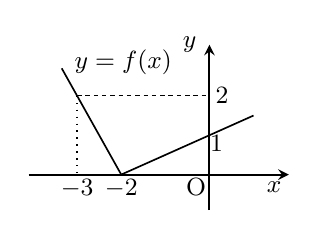
\begin{tikzpicture}[x=0.56cm, y=0.5cm, line width=0.5pt]
  \draw[->, >=stealth, line width=0.7pt] (-4.1,0) -- (1.8,0) node[below left=-1pt, font=\small] {$x$};
  \draw[->, >=stealth, line width=0.7pt] (0,-0.9) -- (0,3.3) node[left=1pt, font=\small] {$y$};
  \node[below left, font=\small, inner sep=1pt] at (0,0) {$\mathrm{O}$};
  % y=f(x): (-2,0) 에서 꺾인 두 반직선
  \draw[line width=0.6pt] (-3.35,2.7) -- (-2,0) -- (1.0,1.5);
  % (-3, 2) 에서 두 축으로 내린 보조선(원문의 점선·파선)
  \draw[dashed, dash pattern=on 1.6pt off 1.4pt, line width=0.4pt] (-3,2) -- (0,2);
  \draw[dotted, line width=0.5pt] (-3,2) -- (-3,0);
  % 라벨(원문 그대로)
  \node[right=1pt, font=\small, inner sep=1pt] at (0,2) {$2$};
  \node[below right=-1pt, font=\small, inner sep=1pt] at (0,1) {$1$};
  \node[below, font=\small, inner sep=1.5pt] at (-3,0) {$-3$};
  \node[below, font=\small, inner sep=1.5pt] at (-2,0) {$-2$};
  \node[right=1pt, font=\small, inner sep=1pt] at (-3.2,2.85) {$y=f(x)$};
\end{tikzpicture}
}\end{minipage}\par
\noindent \dispeq{$\displaystyle\int_{-3}^{1}f(x)\mkern3mu dx$}\par\smallskip\noindent 의 값을 구하시오.
